\documentclass[11pt,a4paper]{article}
\usepackage[margin=2.2cm]{geometry}
\usepackage[T1]{fontenc}
\usepackage{lmodern}
\usepackage{booktabs}
\usepackage{tabularx}
\usepackage{array}
\usepackage{enumitem}
\usepackage{xcolor}
\usepackage{tikz}
\usetikzlibrary{positioning,arrows.meta}
\usepackage[colorlinks=true,linkcolor=blue!50!black,urlcolor=blue!50!black,citecolor=blue!50!black]{hyperref}
\setlist{itemsep=2pt,topsep=4pt}
\newcolumntype{L}{>{\raggedright\arraybackslash}X}

\title{Map-to-Text VLM: Faithful Summaries of Choropleth Maps\\[4pt]\large Midterm Progress Report}
\author{Sarthak Maheshwari (IMT2023014) \and Siddharth Prashant Kini (IMT2023026)}
\date{25 October 2026}

\begin{document}
\maketitle

\begin{center}
\begin{tabularx}{\textwidth}{@{}lL@{}}
\toprule
Code repository & \href{https://github.com/SartMa/choropleth-derenderer}{github.com/SartMa/choropleth-derenderer} (private; team, mentor and GVCL to be added)\\
Weekly slides & \href{https://iiitbac-my.sharepoint.com/:p:/r/personal/sarthak_maheshwari_iiitb_ac_in/_layouts/15/doc2.aspx?sourcedoc=\%7BDCE8C4F7-9DB7-445F-8A17-8A1432DB3F70\%7D}{VLM -- MAPS (OneDrive)}\\
Report period & Start of semester to 25 October 2026\\
\bottomrule
\end{tabularx}
\end{center}

\begin{abstract}
We are building a system that writes accurate text summaries of choropleth maps. It has three stages: a vision-language model (VLM) that reads the map into structured data, a code layer that computes spatial statistics on that data, and a language model that turns the computed facts into prose. Splitting the work this way means no number in a summary is ever generated by guesswork.

At midterm, the first two stages work. The derenderer, Qwen2.5-VL-3B fine-tuned with LoRA on 8 GPU hours, reads US maps with 99.3\% of states in the correct legend range. Magnified tiles of the densest map area, placed by a small learned picker, raised Rhode Island from 47.0\% to 94.4\% and whole-map exact match from 33.1\% to 89.7\%.

On synthetic India maps, accuracy is 79.2\%. Our analysis shows the model reads colours correctly but does not know where Indian states are. When state codes are drawn on the map, big-state accuracy rises from 64\% to 97\%. The code layer gets 16 of 20 controlled test maps fully right. The second half of the semester will train on the full dataset and give the model region positions as input, so it can generalise beyond the US.
\end{abstract}

\section{Introduction and problem statement}
A choropleth map shades each region by a value, such as unemployment by state. People read such maps for patterns: where values are high, which regions cluster, how one area differs from its neighbours. Our goal is to produce long-form summaries of these maps, for single maps and later for collections and time series, where every number and spatial claim is correct.

End-to-end VLMs fall short of this. In our zero-shot baseline on 20 maps of each legend type, Qwen2.5-VL-7B produced valid output for only 35\% of discrete-legend maps, with no state values recovered. InternVL3-8B produced valid output for 55\%, covering 36\% of states. Chart-to-text models such as VisText and Chart-to-Text do not transfer either: they have no notion of regions, neighbours or continuous colour legends.

We therefore split the problem into three stages (Figure~\ref{fig:pipeline}):
\begin{enumerate}
\item \textbf{Derenderer (VLM).} Reads one map image into one JSON record: the title, the legend text and type, and a value or legend range for every region. Its only job is perception.
\item \textbf{Code layer (deterministic).} Builds a region adjacency graph from real boundaries and computes spatial statistics: global and local Moran's I, Getis-Ord Gi*, trend surfaces, and later emerging hot-spot analysis over time. These are executed code, so they cannot hallucinate.
\item \textbf{Narrator (LLM).} Chooses which computed facts matter and phrases them. It never does arithmetic itself.
\end{enumerate}

\begin{figure}[h]
\centering
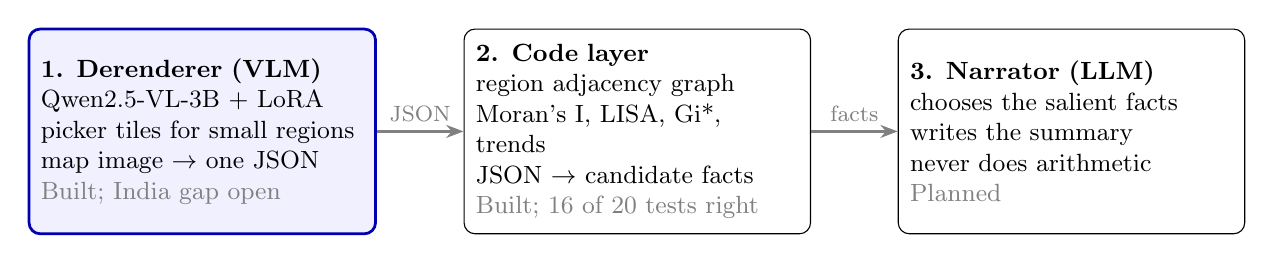
\begin{tikzpicture}[
  stage/.style={draw, rounded corners=4pt, minimum width=4.4cm, minimum height=2.6cm, align=left, font=\small, text width=4.1cm},
  arr/.style={-{Stealth[length=2.2mm]}, thick, gray}]
\node[stage, draw=blue!70!black, fill=blue!6, line width=1pt] (d) {\textbf{1. Derenderer (VLM)}\\ Qwen2.5-VL-3B + LoRA\\ picker tiles for small regions\\ map image $\to$ one JSON\\ \textcolor{gray}{Built; India gap open}};
\node[stage, right=1.1cm of d] (c) {\textbf{2. Code layer}\\ region adjacency graph\\ Moran's I, LISA, Gi*, trends\\ JSON $\to$ candidate facts\\ \textcolor{gray}{Built; 16 of 20 tests right}};
\node[stage, right=1.1cm of c] (n) {\textbf{3. Narrator (LLM)}\\ chooses the salient facts\\ writes the summary\\ never does arithmetic\\ \textcolor{gray}{Planned}};
\draw[arr] (d) -- node[above, font=\footnotesize, text=gray] {JSON} (c);
\draw[arr] (c) -- node[above, font=\footnotesize, text=gray] {facts} (n);
\end{tikzpicture}
\caption{The three-stage pipeline and the status of each stage at midterm. Only the derenderer reads pixels; the numbers are computed by code.}
\label{fig:pipeline}
\end{figure}

This report covers the derenderer in detail, since most of the semester's work went there, and summarises the code layer's first tests.

\section{Related work}
Our pipeline follows the tool-augmented line of chart understanding: extract the data first, then reason over it with code or a language model.

\begin{center}
\small
\begin{tabularx}{\textwidth}{@{}l L L@{}}
\toprule
Work & What it does & What we take from it\\
\midrule
Pix2Struct~\cite{pix2struct} & End-to-end image-to-text transformer & End-to-end models drop regions and hallucinate numbers on thematic maps\\
MatCha~\cite{matcha} & Pretrains Pix2Struct on chart derendering and math reasoning & Derendering as a training target\\
DePlot~\cite{deplot} & Converts a plot to a table, then an LLM reasons over it & The two-step design our pipeline extends to maps\\
TinyChart~\cite{tinychart} & 3B model that writes Python for its arithmetic & Hand numerical work to executed code\\
MapQA~\cite{mapqa} & Choropleth question answering over US maps & Our main training and test data\\
MAPWise~\cite{mapwise} & 3,000 map questions over US, India and China maps & Humans still beat all VLMs on map reasoning\\
ChartQA~\cite{chartqa} & 32.7K chart questions needing arithmetic & Models struggle beyond template extraction\\
Chart-to-Text~\cite{chart2text}, VisText~\cite{vistext} & Chart images with data tables and human summaries & Summary styles and caption levels for the narrator\\
\bottomrule
\end{tabularx}
\end{center}

From the readings the professor suggested, two ideas carry over. Hard-negative contrastive training (Liu et al.) could sharpen colour discrimination between near-identical legend shades. AG-CAM heatmaps (Dong and Crisan) could show which pixels the model used for each region, as a diagnostic.

The professor also pointed us to multi-scale backbones (Swin, Mask2Former, FPN) and to GeoAI foundation models for boundary recognition. We tested the cheap model-level version of multi-scale (S2~\cite{s2} and feature fusion, Section~\ref{sec:method}). Boundary-aware foundation models are now directly relevant, given the India findings in Section~\ref{sec:india}.

\section{Datasets}
We train and test on one public dataset and two synthetic ones we built; every map has exact per-region ground truth.

\begin{center}
\small
\begin{tabularx}{\textwidth}{@{}l r r r l L@{}}
\toprule
Dataset & Train & Dev & Test & Regions & Ground truth\\
\midrule
MapQA-S (converted) & 12,470 & 4,155 & 4,157 & 50 US states & MapQA's data tables, its own split by map\\
Synthetic US & 9,938 & 994 & 997 & 50 US states & Our generator\\
Synthetic India & 9,845 & 980 & 981 & 32 states and UTs & Our generator\\
\bottomrule
\end{tabularx}
\end{center}

\textbf{MapQA-S} is a set of US choropleths in a few fixed rendering styles. We convert each map into one target JSON: title, legend title, legend type (continuous or discrete), data type (percentage or number), the legend ranges for discrete maps, and a value or range index per state code.

\textbf{The synthetic generator} draws real boundaries from geoBoundaries~\cite{geoboundaries} and randomises the palette, legend type and position, number of bins, fonts, border style, image size, JPEG compression, missing data, and whether region codes are printed (40\% of maps). Values follow random spatial patterns, including clustered ones. Each map passes a pixel check that every listed region shows its colour. For India, four union territories (Lakshadweep, Chandigarh, Puducherry, Dadra and Nagar Haveli and Daman and Diu) are drawn but not scored, because at our resolution they cover 0.3 to 20 pixels. Delhi, at about 60 pixels, is the smallest scored region.

\textbf{The CMA dataset} shared by the professor contains about 150 real Indian choropleths and 10,000 US maps. Its labels cover legend type, component boxes (title, map, legend) and state outlines, but not per-state values or legend ranges. We can use its India maps to check where our tile picker looks on real map styles, but not to measure derendering accuracy. The professor has asked the dataset's authors for the source tables, which would make it a real-map test set.

\section{Method: the derenderer}\label{sec:method}
The derenderer is Qwen2.5-VL-3B-Instruct~\cite{qwen25vl} fine-tuned with LoRA~\cite{lora} to emit one JSON record per map; small regions are handled by adding magnified tiles of the map as extra images.

\textbf{Model and training.} LoRA rank 16 on the language model and the vision tower's MLP layers trains 37M of 3.8B parameters. Training runs in fp16 on one Kaggle T4 (16 GB), batch 1 with 16-step gradient accumulation, learning rate $2\times10^{-4}$ with warm-up and cosine decay, and images capped at 640,000 pixels. A launcher script packs the code into a Kaggle notebook, pushes it from the command line and downloads the results. The base adapter was trained for 8 hours on MapQA-S and synthetic US maps; later runs continue from it.

\textbf{Output format.} Regions are keyed by their codes (\texttt{"RI": 3}) rather than listed in a fixed order, so one skipped value cannot shift every later one, and the same format works for any country. Discrete maps give the index of the legend range; continuous maps give the number read off the colour bar; missing data gives null.

\textbf{The small-region problem.} Each vision token covers a $28\times28$-pixel square of the map. Rhode Island and Delaware are smaller than one token, so their colour is mixed with their neighbours' before the language model sees it. After 8 hours of training, Rhode Island and Delaware caused 73\% of all discrete-legend errors, and more training did not reduce this.

\textbf{Approaches we tried for small regions:}
\begin{enumerate}
\item \textbf{Hand-measured crop.} A fixed magnified crop of the US north-east as a second image. It helped Delaware by about 10 points but was measured for one US layout.
\item \textbf{Rule-based tiles.} A rule finds every region smaller than one token, then places two square windows (about 14\% of the map width) where those regions are densest. Each window is magnified $3\times$ and passed as an extra image, with its position on the map stated in the prompt. Training randomly drops the tiles 20\% of the time.
\item \textbf{Learned tile picker (MLP).} A small network ($2048 \to 256 \to 1$ per token) reads the vision tokens the model already computes and predicts how many small regions sit under each token. It is trained with a Poisson loss on the rule's counts from 1,800 maps, in minutes, without retraining the VLM. Its counts choose the tiles at test time.
\item \textbf{CNN picker.} The same task with $3\times3$ convolutions over the token grid, so each token sees about $7\times7$ neighbours (0.56M weights against the MLP's 0.52M).
\item \textbf{Model-level multi-scale} (the professor's suggestion): \textbf{S2} runs the vision tower on the whole map at $2\times$ and averages the fine features into the normal tokens; \textbf{fusion} adds tile features into the map's own tokens through new trainable layers, so the token count does not grow.
\end{enumerate}

\section{Experiments and results on US maps}
Tiles placed by the learned MLP picker give the best US results: 89.7\% of discrete maps fully correct and Rhode Island right 94.4\% of the time, up from 33.1\% and 47.0\%.

All comparisons below use the same 400 MapQA test maps (302 discrete, 98 continuous), drawn once at random and never trained on. Every model reads the same prompt and is scored the same way: discrete maps by whether each state gets the right legend range, continuous maps by the error as a share of the legend's range (nMAE).

\textbf{Base fine-tune (8 hours, 8,784 maps seen, 39\% of one pass).} On every map the output was valid JSON, with all 50 states, the right title, legend title and data type. Legend ranges were copied exactly on 99.0\% of discrete maps and 97.8\% of states fell in the right range. On continuous maps the average error was 4.1\% of the range, with 85.0\% of states within 5\%. On synthetic US maps the same model scored 97.3\% and 3.5\%.

\begin{table}[h]
\centering\small
\caption{Discrete maps, by strategy (302 MapQA test maps).}
\begin{tabular}{@{}lrrrr@{}}
\toprule
Strategy & States in right range & Whole map exact & Rhode Island & Delaware\\
\midrule
Baseline (no tiles) & 97.8\% & 33.1\% & 47.0\% & 74.2\%\\
Fusion & 97.3\% & 26.5\% & 47.0\% & 76.8\%\\
Rule-based tiles (7 h) & 99.1\% & 79.8\% & 83.8\% & 95.7\%\\
MLP picker tiles (7 h) & \textbf{99.3\%} & \textbf{89.7\%} & \textbf{94.4\%} & \textbf{96.4\%}\\
\bottomrule
\end{tabular}
\end{table}

\begin{table}[h]
\centering\small
\caption{Continuous maps, by strategy (98 MapQA test maps). Errors are a share of the legend's range.}
\begin{tabular}{@{}lrrrrr@{}}
\toprule
Strategy & nMAE & nRMSE & Within 5\% & RI error & DE error\\
\midrule
Baseline (no tiles) & 4.12\% & 6.77\% & 85.0\% & 25.9\% & 12.9\%\\
Fusion & 3.45\% & 6.38\% & 81.6\% & 25.9\% & 10.5\%\\
Rule-based tiles (7 h) & 3.31\% & 4.32\% & 90.0\% & 7.5\% & 4.8\%\\
MLP picker tiles (7 h) & \textbf{3.24\%} & \textbf{3.98\%} & \textbf{90.4\%} & \textbf{5.5\%} & \textbf{4.6\%}\\
\bottomrule
\end{tabular}
\end{table}

\textbf{What each change did, on the same weights:}
\begin{itemize}
\item \textbf{Tiles on vs off:} 125 Rhode Island answers fixed, 5 broken. The tiles are what fix small states.
\item \textbf{Learned picker vs the rule it learned from:} 38 fixed, 6 broken. The picker beats its own teacher, although its tiles hold fewer small regions (68\% vs 79\%). We do not yet know why.
\item \textbf{Zoom matters, tile count does not:} Rhode Island was right 59.9\% of the time at $2\times$ zoom and 80.8\% at $3\times$. One, two or three tiles made little difference, since US small states sit in one cluster.
\item \textbf{More training alone, without tiles:} no significant change. The information is lost in the image tokens.
\item \textbf{Model-level multi-scale did not learn in our budget.} S2 reached 41.7\% on Rhode Island; fusion stayed at 47.0\% even after a retry with a $10\times$ learning rate. Both add millions of new weights that learn only through the final JSON answer, and 100--200 updates were not enough.
\end{itemize}

\textbf{Does the picker memorise where the US north-east is?} We showed it the same maps mirrored and flipped, without retraining (Table~\ref{tab:probe}).

\begin{table}[h]
\centering\small
\caption{Share of a map's small regions inside the two tiles, 200 maps per row.}
\label{tab:probe}
\begin{tabular}{@{}lrrr@{}}
\toprule
Maps shown & Rule's tiles hold & MLP picker's tiles hold & Picker's first tile top-right\\
\midrule
US, as drawn & 79\% & 68\% & 100\%\\
US, mirrored left-right & 76\% & 68\% & 0.5\%\\
US, flipped top-bottom & 71\% & 61\% & 2\%\\
US, rotated 180\textdegree & 71\% & 63\% & 0\%\\
India, never seen by the picker & 64\% & 53\% & 99\%\\
\bottomrule
\end{tabular}
\end{table}

The MLP's tiles move with the small states and keep a steady gap of about 10 points to the rule. The CNN picker fitted its training data better (held-out loss 0.0239 vs 0.0285) but memorised positions: on flipped maps its tiles held only 23\% of small regions, and end to end it got Rhode Island right 88.4\% of the time against the MLP's 94.4\%. We kept the MLP. The S2 figure comes from an earlier run on a smaller test subset, so compare it loosely.

\section{India: the model reads colours but does not know Indian geography}\label{sec:india}
On India maps, 79.2\% of states land in the right range, and the cause of the gap is geography: with state codes drawn on the map, big-state accuracy rises from 64\% to 97\%.

The 7-hour model had 1,000 synthetic India maps in its training pool but saw only about 200 of them, once each. We tested it on 100 synthetic India maps (43 discrete, 57 continuous).

\begin{center}
\small
\begin{tabular}{@{}lrr@{}}
\toprule
Test set & Discrete: states in right range & Continuous: nMAE\\
\midrule
US (MapQA) & 99.1\% & 0.033\\
Synthetic US, same generator as India & 99.5\% & 0.029\\
Synthetic India & 79.2\% & 0.134\\
\bottomrule
\end{tabular}
\end{center}

Synthetic US maps from the same generator score 99.5\%, so the drop is not caused by the drawing style.

\textbf{Where it fails.} The small regions are weakest: Delhi 42--47\%, Goa 40--44\%, Tripura 37--40\%, Sikkim 33--43\% and Andaman and Nicobar 44--49\% on discrete maps (ranges across tile settings). But large interior states also fail: Chhattisgarh 60\%, Bihar 63\%, Telangana 65\%. Rajasthan and Gujarat, with distinctive shapes on the edge, are at 100\%.

\textbf{Tiles do not help on India.} Discrete accuracy stays within half a point whether we use no tiles, the rule's tiles, the MLP picker or the CNN picker. The picker sends its first tile to the north-east cluster on 96--99\% of maps and never to Delhi or Goa. The rule also discards patches under 40 pixels as specks, and the borders leave Delhi near that size.

\textbf{Errors copy a neighbour's colour.} We took every wrong discrete answer where the state's neighbours and the map's average pull in opposite directions. In 33 of 40 such cases (31 of 42 with tiles), the wrong answer moved toward the neighbours' colour. The model reads a real colour, but from the region next door.

\textbf{Probe: give the model the region names.} The generator prints region codes on 40\% of maps, which the model also saw in training. On the 100 test maps, those with codes drawn score 86\% against 61\% without (continuous error 0.078 vs 0.174). On US maps, codes make no difference (98.6\% vs 98.7\%), because the model already knows the US layout. To remove any difference between maps, we redrew 20 India test maps from the same random draws with and without codes (Table~\ref{tab:labels}).

\begin{table}[h]
\centering\small
\caption{Paired probe: the same 20 India maps with and without region codes.}
\label{tab:labels}
\begin{tabular}{@{}lrr@{}}
\toprule
 & Plain map & Codes drawn\\
\midrule
Big states, discrete: right range & 63.9\% & \textbf{97.3\%}\\
Big states, continuous: error as share of range & 0.152 & \textbf{0.054}\\
Small regions (never labelled), discrete & 36\% & 40\%\\
Small regions, continuous error & 0.253 & 0.225\\
\bottomrule
\end{tabular}
\end{table}

Every weak big state reached 100\% with codes (Chhattisgarh from 20\%, Bihar from 33\%, Jharkhand from 50\%). The generator never prints codes on the five smallest regions, so whether they suffer from geography or from resolution is still open.

A second probe outlined one state in magenta and named it in the prompt. Accuracy on the outlined state fell, even for Rajasthan (100\% to 30\%), while other states were unaffected. The model never saw outlines in training, so this probe needs a model trained with them before it can tell us anything.

\textbf{What this means.} Our US results reflect a model that has learned the US layout, not map reading in general. Telling the model where each region is recovers nearly all of the India gap for big states with no extra India training. This is the direction for the second half: give region positions as input, so the derenderer transfers to any country with a boundary file.

\section{Code layer (stage 2)}
The first version of the code layer is implemented and gets 16 of 20 controlled test maps fully right; its misses are all very small clusters or single outliers.

It builds a US state adjacency graph from real boundaries (shared borders are edges), then runs global Moran's I, local Moran's I (LISA), Getis-Ord Gi* and trend-surface regression, and compares an extreme value against its field. We tested it on 20 maps with known planted patterns.

\begin{center}
\small
\begin{tabularx}{\textwidth}{@{}l L L@{}}
\toprule
Cases & Planted pattern & Result\\
\midrule
1, 2, 4, 15 & South, West or Mountain states high; Midwest low & Found and labelled with the right region name\\
3 & New England high & 2 of 6 states significant, labelled ``part of'' rather than overclaimed\\
5, 6, 12, 16 & Pure noise, all equal, checkerboard & Correctly reported no pattern\\
7, 8 & West-to-east and south-to-north gradients & Trend found in the right direction\\
13, 14 & An offshore state much higher; a hotspot with missing data & Correct, including the missing-state list\\
17 & Discrete map, South in the top band & Hotspot found on banded data\\
19, 20 & An extreme value that agrees or disagrees with its field & Both classified correctly\\
10 & Two separate hotspots (South, and Washington with Oregon) & South found, the two-state pair missed\\
9, 11, 18 & One outlier (Texas); a two-state cluster (Alabama, Mississippi); two tiny states (RI, CT) & Missed\\
\bottomrule
\end{tabularx}
\end{center}

The misses share a cause: hotspot statistics need a few neighbouring regions to reach significance, so one or two states cannot. A separate check for single outliers is one way to cover these cases. Once the derenderer is trained on the full data, the two stages will be joined and tested end to end on maps whose true values we know.

\section{Limitations and open questions}
\begin{itemize}
\item \textbf{Undertrained.} The best model saw about 21\% of one pass over the training data, by the training log's count (313 updates of 16 maps). All results are from Kaggle's 30-hour weekly GPU limit.
\item \textbf{A 400-map test sample.} The paired comparisons are solid, but absolute numbers will move a little on the full 4,157-map MapQA test set.
\item \textbf{Synthetic India only.} We have no real India maps with per-state values yet.
\item \textbf{Small Indian regions.} Delhi, Goa, Sikkim, Tripura and Andaman stay near 40\%. Codes are never drawn on them, so we cannot yet tell geography from resolution.
\item \textbf{Why the picker beats its teacher} is unexplained: its tiles hold fewer small regions than the rule's, yet it scores better.
\item \textbf{Scaled units.} On a colour bar labelled in millions, the model can drop the scale (3.63 instead of 3,630,000). One such map moves the continuous average from 3.1\% to 4.1\%.
\item \textbf{No-data regions.} In the base model, 61 grey no-data states were given a range.
\item \textbf{Model-level multi-scale} (S2, fusion) was tested only at a cheap scale; a full multi-scale backbone was beyond our compute.
\end{itemize}

\section{Plan for the second half}
The next step is one full training run on lab GPUs, followed by giving the model region positions so it generalises beyond the US.
\begin{enumerate}
\item \textbf{Full training run.} MLP-picker tiles at $3\times$ zoom, trained on all of MapQA-S plus synthetic US and India maps for 2--3 passes, scored on the full MapQA test set.
\item \textbf{Region positions as input.} Give the model where each region is (codes on the map, label points or a region-ID map from the boundary file), train with it, and test on India and on a country it has never seen.
\item \textbf{Small regions everywhere.} Extend the India probe to codes on the smallest regions, and teach the picker from true positions of small regions rather than from the hand-written rule, possibly pretrained on generated random-polygon maps.
\item \textbf{Real-map evaluation.} Score the derenderer on real India maps once the CMA source tables arrive.
\item \textbf{End-to-end pipeline.} Join the derenderer and the code layer, cover single-state outliers, add the narrator, and evaluate the summaries for factual accuracy (numerical consistency checks and question-based verification) as well as fluency.
\end{enumerate}

\textbf{Compute requirements}, already sent to the professor:
\begin{center}
\small
\begin{tabularx}{\textwidth}{@{}lL@{}}
\toprule
Resource & Need\\
\midrule
Training time & About 16 Kaggle T4 hours per pass over 23,408 maps; 40--60 T4 hours for 2--3 passes, less on faster GPUs\\
GPU memory & At least 16 GB\\
System RAM & About 32 GB\\
Disk & About 50 GB free\\
Network & Internet once, to download the Qwen weights\\
\bottomrule
\end{tabularx}
\end{center}

\begin{thebibliography}{99}\small
\bibitem{chartqa} A. Masry et al. ChartQA: A Benchmark for Question Answering about Charts with Visual and Logical Reasoning. 2022. \url{https://arxiv.org/abs/2203.10244}
\bibitem{pix2struct} K. Lee et al. Pix2Struct: Screenshot Parsing as Pretraining for Visual Language Understanding. 2022. \url{https://arxiv.org/abs/2210.03347}
\bibitem{matcha} F. Liu et al. MatCha: Enhancing Visual Language Pretraining with Math Reasoning and Chart Derendering. 2022. \url{https://arxiv.org/abs/2212.09662}
\bibitem{deplot} F. Liu et al. DePlot: One-shot Visual Language Reasoning by Plot-to-Table Translation. 2022. \url{https://arxiv.org/abs/2212.10505}
\bibitem{tinychart} L. Zhang et al. TinyChart: Efficient Chart Understanding with Visual Token Merging and Program-of-Thoughts Learning. 2024. \url{https://arxiv.org/abs/2404.16635}
\bibitem{mapwise} S. Mukhopadhyay et al. MAPWise: Evaluating Vision-Language Models for Advanced Map Queries. 2024. \url{https://arxiv.org/abs/2409.00255}
\bibitem{mapqa} S. Chang et al. MapQA: A Dataset for Question Answering on Choropleth Maps. \url{https://github.com/OSU-slatelab/MapQA}
\bibitem{qwen25vl} S. Bai et al. Qwen2.5-VL Technical Report. 2025.
\bibitem{lora} E. Hu et al. LoRA: Low-Rank Adaptation of Large Language Models. 2021.
\bibitem{s2} B. Shi et al. When Do We Not Need Larger Vision Models? 2024.
\bibitem{chart2text} S. Kantharaj et al. Chart-to-Text: A Large-Scale Benchmark for Chart Summarization. 2022.
\bibitem{vistext} B. Tang et al. VisText: A Benchmark for Semantically Rich Chart Captioning. 2023.
\bibitem{geoboundaries} geoBoundaries: open database of political administrative boundaries. \url{https://www.geoboundaries.org}
\bibitem{readings} Readings suggested by the professor: \url{https://aclanthology.org/2024.findings-naacl.62.pdf}; \url{https://arxiv.org/abs/2502.17589}; \url{https://aclanthology.org/2025.findings-emnlp.573.pdf}; \url{https://ieeexplore.ieee.org/abstract/document/11261397}; Opportunities and Challenges of Foundation Models for GeoAI.
\end{thebibliography}

\end{document}
